\section{Measurement with back-light illumination}
To measure the size and form of an object there are multiple ways. A popular way to get the contour is to place a light source behind the object desired to measure, and aim on the object with an camera. With this method the optical sensors get the silhouette of the object. 
\subsection{Short introduction to photometry}
Photometry is the science concerned with the electromagnetic radiation visible to the human eye. In this section some important basics used further in this paper are explained. The theories of the following sections were taken from the textbook Physik 2 \cite{ruh}
\subsubsection{Photometric quantities}
In principle the normal physical quantities and units such as watts and joules could be used for the measurements of light radiation. However, in order to take into account the spectral sensitivity of the human eye, special photometric quantities and units are introduced. 

\begin{tabular}{ |lc|lc|  }
	\hline
	\multicolumn{2}{|c|}{Quantity}&\multicolumn{2}{|c|}{Unit} \\
	\hline\hline
	\multicolumn{1}{|c|}{Name}			& \multicolumn{1}{|c|}{Symbol}	& \multicolumn{1}{|c|}{Name}	& \multicolumn{1}{|c|}{Symbol}\\

	\hline
	Luminous flux		& $\phi_v$	& lumen		& lm\\
	Luminous intensity 	& $I_v$ 	& candela	& cd\\
	Luminance			& $L_v$		& candela/$\text{m}^2$	& cd/$m^2$\\
	Illuminace 			& $E_v$ 	& lux (=lumen/$\text{m}^2$) 	& lx\\

	\hline
\end{tabular}
\subsubsection{Light source}
To model a light source it is assumed that the source is a very small point which emits the light rays in all directions. The density of the light rays is reduced with the factor $\frac{1}{r^2}$ with $r$ being the distance. Intensity of the light is proportional to the density of the rays. This behavior has to do with the fact that the surface area $A$ of a sphere
\begin{align*}
A=\int_{0}^{2 \pi} \int_{0}^{\pi} r^{2} \sin \theta d \theta d \varphi=4 \pi r^{2}
\end{align*}
grows squared with the distance from the center $r$.
\begin{align*}
A = 4\pi r^2
\end{align*}
The intensity of light in photometry 
\begin{figure}[ht]
	\centering
	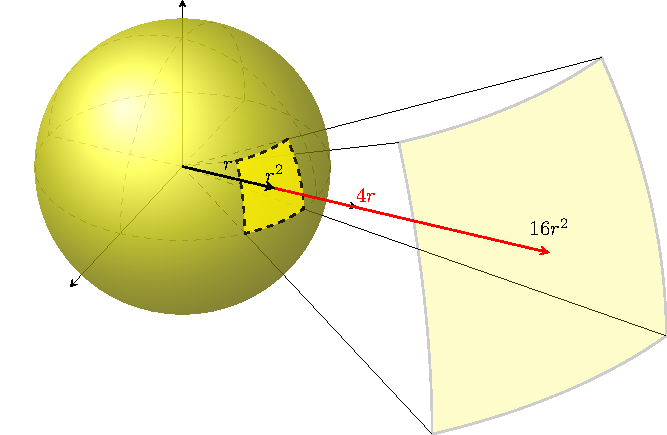
\includegraphics[width=0.6\textwidth]{2-theory/backlight/light.pdf}
	\caption{Light source in 3d\label{theory:light}}
\end{figure} 


\subsubsection{Light ray distribution}
\begin{figure}[ht]
	\centering
	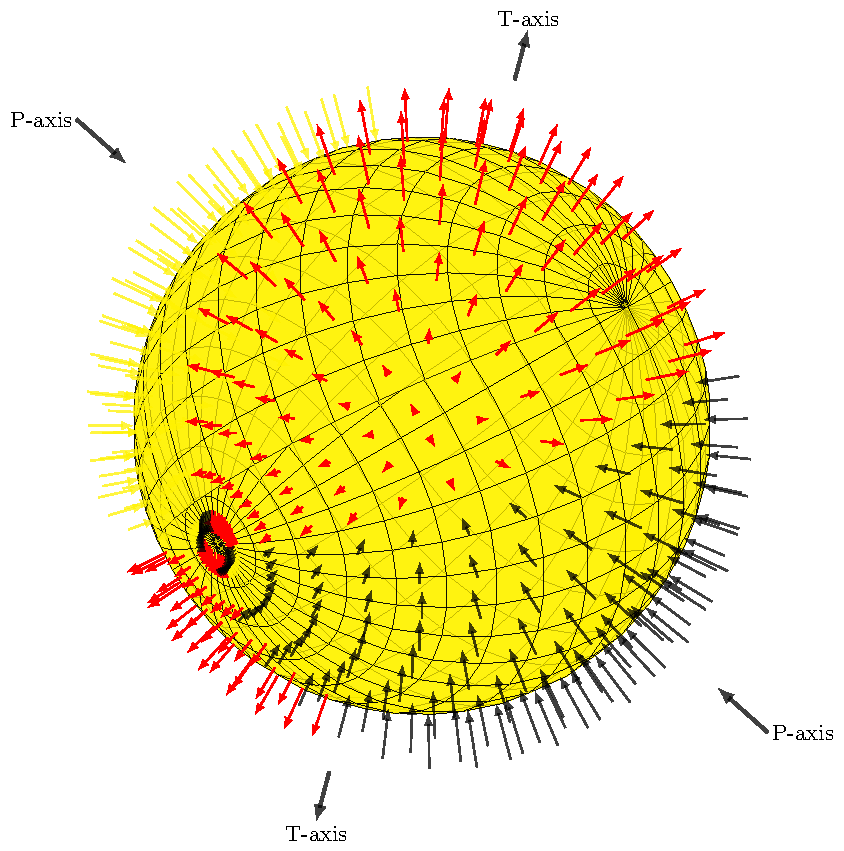
\includegraphics[width=1\textwidth]{2-theory/backlight/lightsource.pdf}
	\caption{Light distribution\label{theory:lightdistribution}}
\end{figure} 
\subsubsection{Light properties}
\subsection{Measurement precision changes}
\subsection{Image sensor properties}

